\chapter{Data Extraction and Visualization - EU Stats}

\section{Introduction and the Datasets Chosen}
\paragraph{ }The datasets used for this task were both taken from the Eurostat portal. Links to download the data can be found in the `README' text file found in the data folder provided for this task. The data chosen where Malta ranks surprisingly well is that of the number of healthy life years. According to the eurostat website, healthy life years measures the number of years that a person at birth is still expected to live in a healthy condition. The data chosen were Malta ranks surprisingly bad is the employment rate data, specifically the female employment rate.

\section{Healthy Life Years}
\paragraph{ }Since 2006, the number of healthy life years has increased from 69.5 years to 72.4 years for females and from 68.3 years to 71.1 years for Males, however this increase has not been linear. In fact, when looking at Figure \ref{fig::hly_timeseries} we can note that the number of healthy life years in Malta peaked for both males and females in 2015. Since 2015, the healthy life years for females has dropped by by 2.2 years while that of males has dropped by 1.5 years. An interesting study would be to determine the source of this decrease and to answer the question \textit{``Will this value continue to decrease in the future?"} 

\paragraph{ }Surprisingly, when comparing the Maltese Data to the rest of the EU, Malta ranked the second best in 2016 when it comes to healthy life years, being only beaten by Sweden with an average healthy life years value of 73.15 years (where Malta's average healthy life years value is 71.75). Figure \ref{fig::hly_bar} shows the top 10 countries in the EU with the highest healthy life years expected value.

\begin{figure}[!t]
	\begin{minipage}[b]{0.45\linewidth}
		\centering
		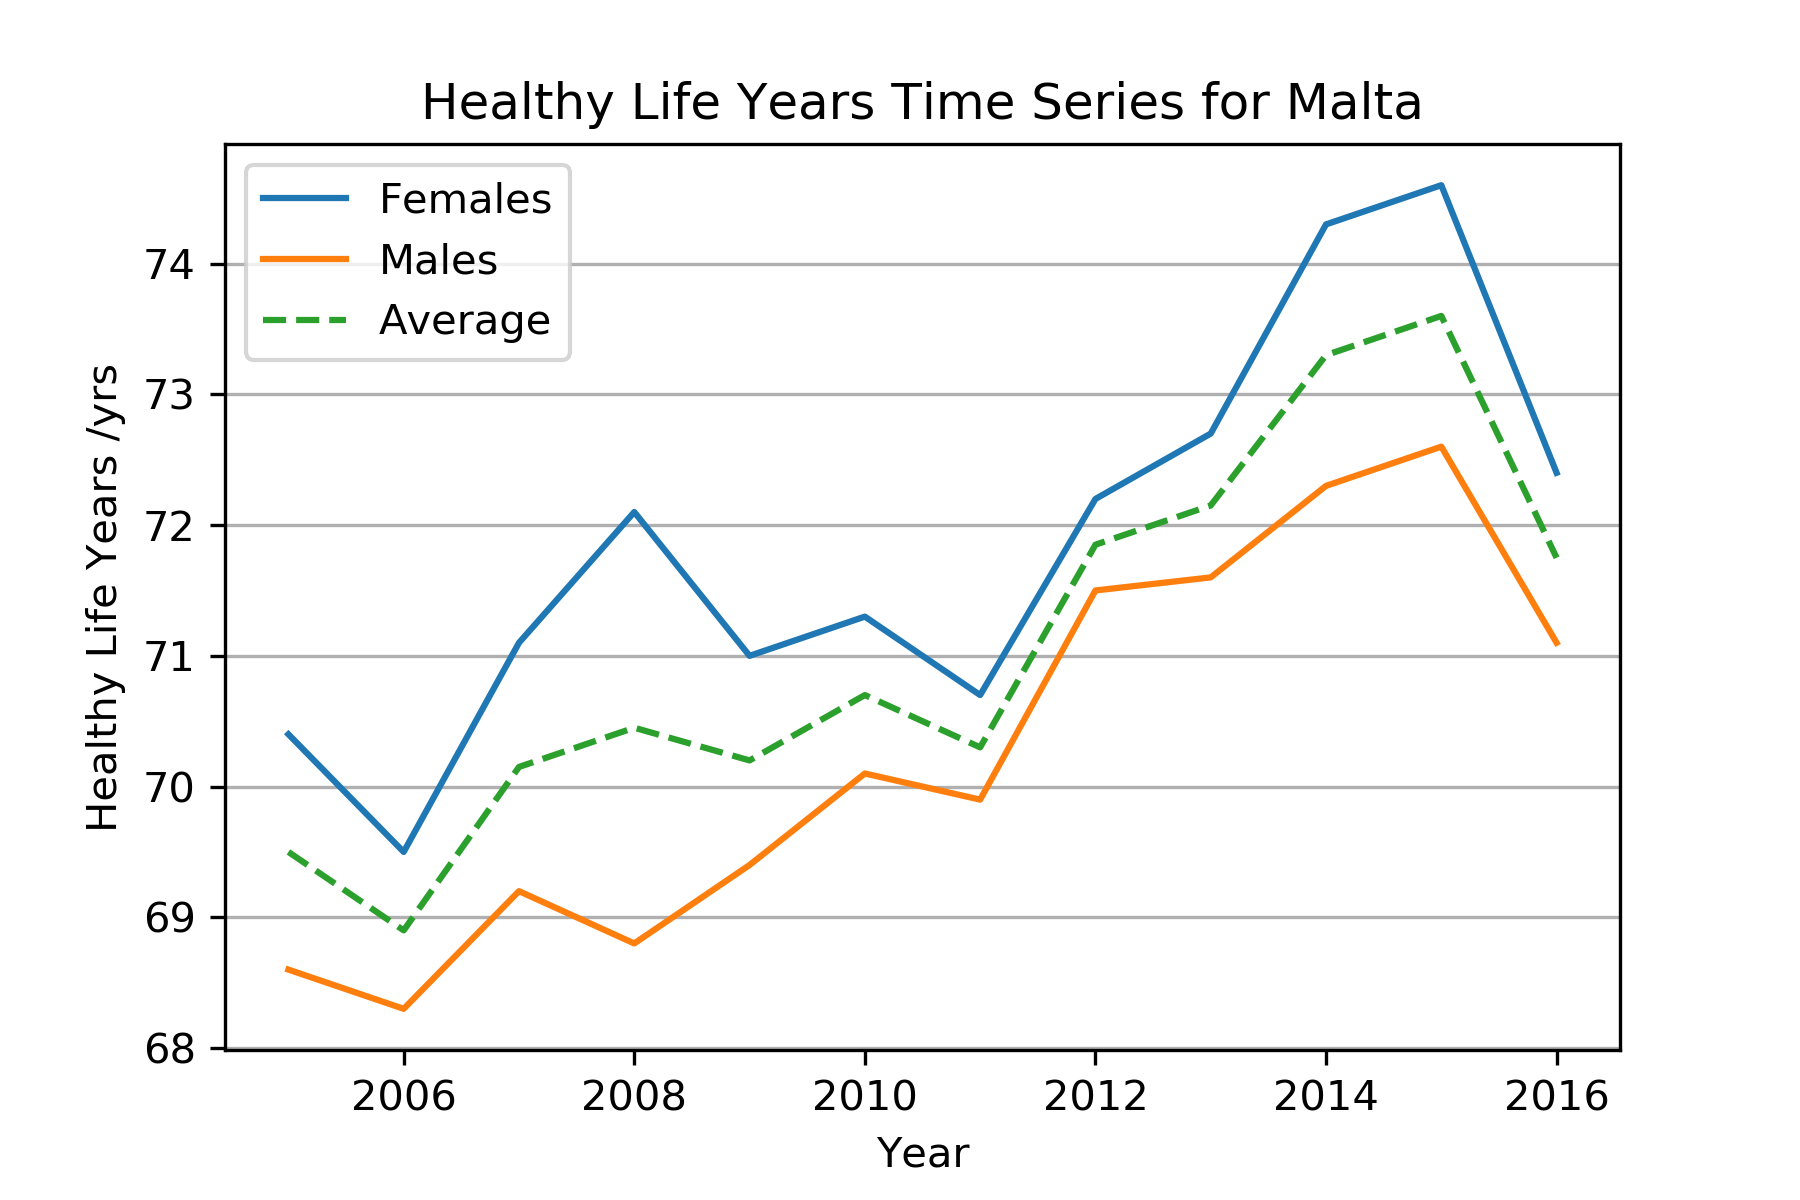
\includegraphics[width=\textwidth]{hly_time_series}
		\caption[Healthy Life Years in Malta]{Time Series Plot showing Malta's Expected Healthy Life Years}
		\label{fig::hly_timeseries}
	\end{minipage}	
	\hspace{0.5cm}
	\begin{minipage}[b]{0.45\linewidth}
		\centering
		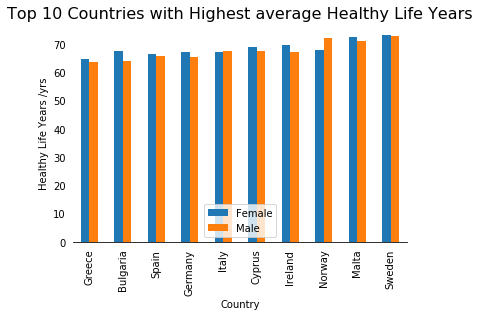
\includegraphics[width=\textwidth]{hly_bar_chart}
		\caption[Top Healthy Life Years in the EU]{Top 10 EU States with the Highest Expected Healthy Life Years}
		\label{fig::hly_bar}
	\end{minipage}	
\end{figure}  

\section{Employment Rate}
\paragraph{ }Sine 2005, the employment rate in Malta has been on a nearly constant increase, having only dipped slightly in 2009. In particular when looking at the time series plot for the employment rate in Malta (Figure \ref{fig::er_timeseries}) we can note that since 2009, female employment rate has increased significantly. The rate of this change has also increased but although this is a positive step in the right direction, these numbers are not too good when compared to other EU States. In fact, as can be seen in Figure \ref{fig::er_bar}, Malta ranks in the top 10 worst countries for female employment rate!

 \begin{figure}[!b]
 	\begin{minipage}[b]{0.45\linewidth}
 		\centering
 		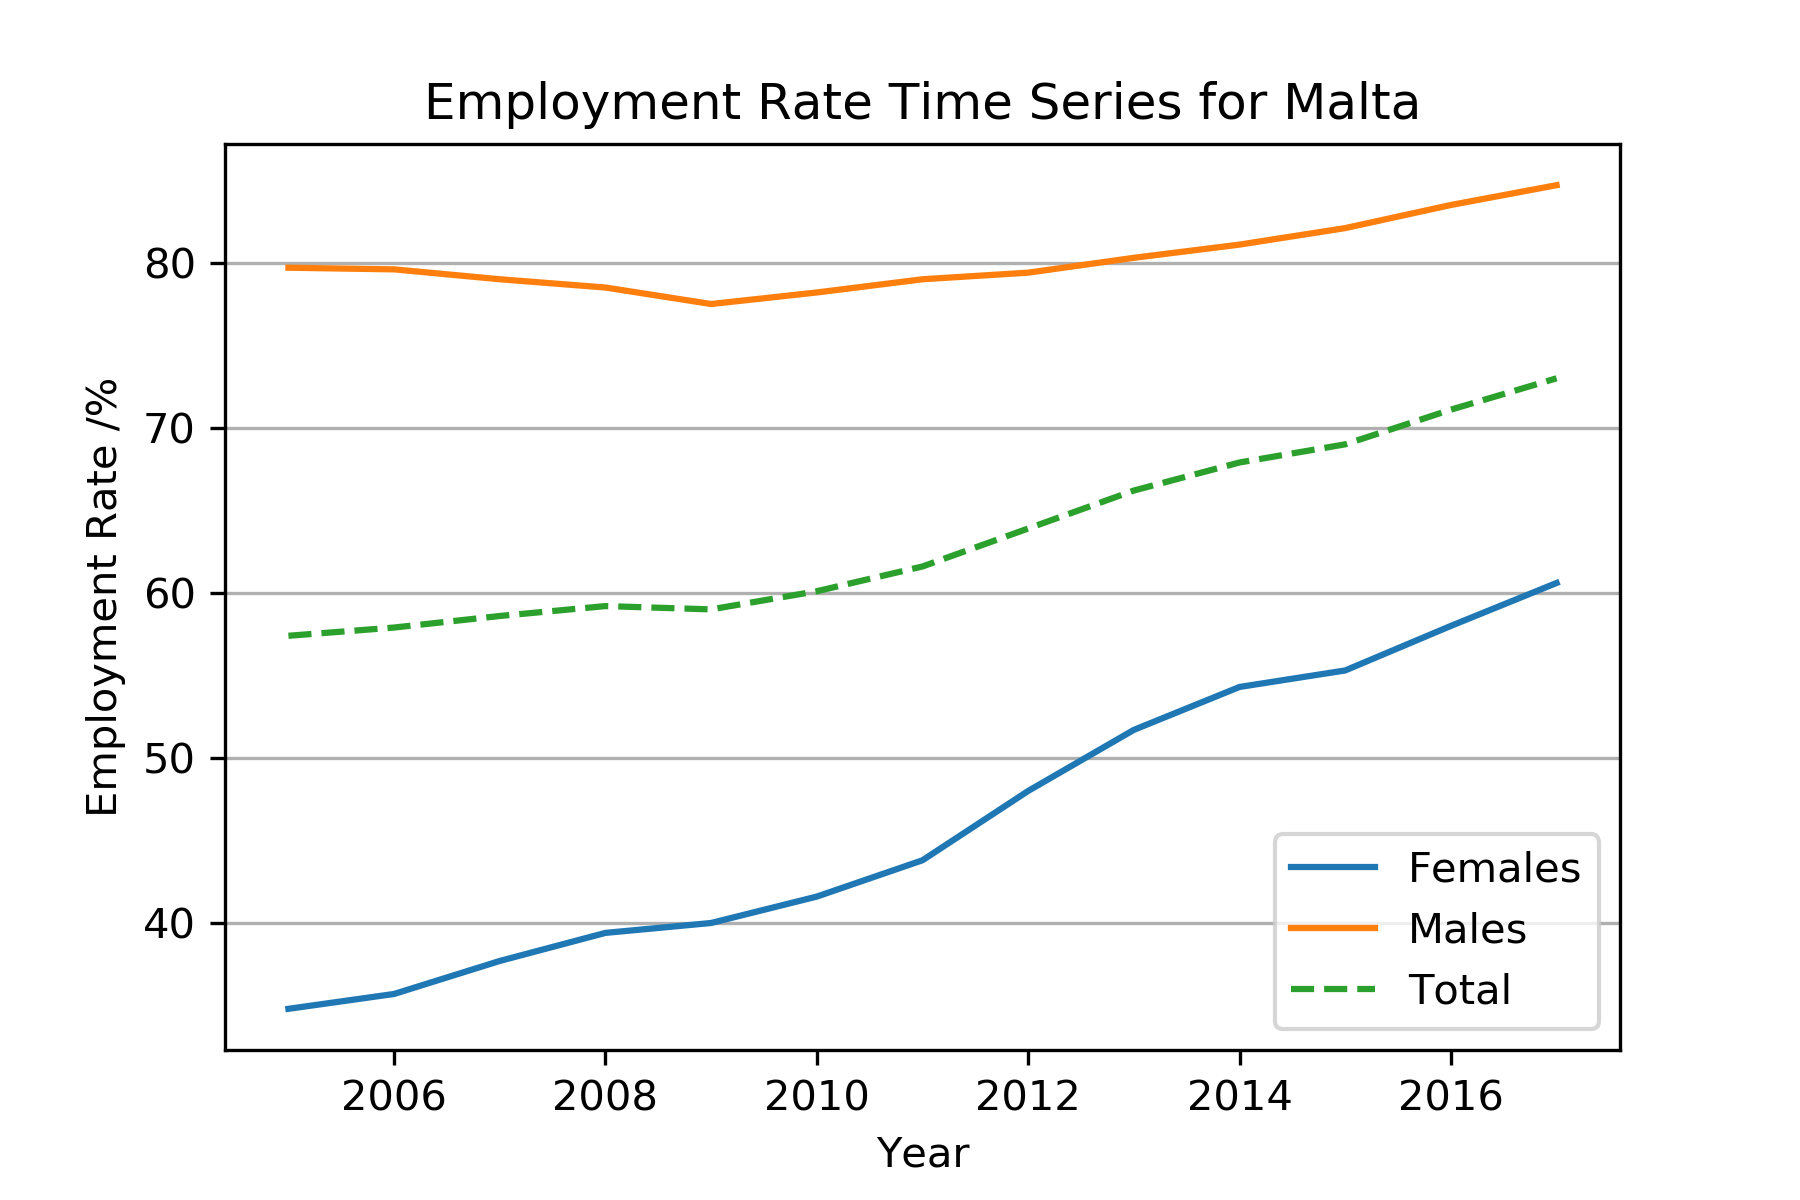
\includegraphics[width=\textwidth]{er_time_series}
 		\caption[Employment Rate in Malta]{Time Series Plot showing Malta's Employment Rate}
 		\label{fig::er_timeseries}
 	\end{minipage}	
 	\hspace{0.5cm}
 	\begin{minipage}[b]{0.45\linewidth}
 		\centering
 		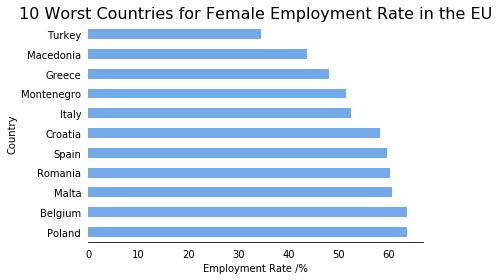
\includegraphics[width=\textwidth]{er_bar_chart}
 		\caption[Worst Employment Rate Values in the EU]{Top 10 worst EU States for Employment Rates}
 		\label{fig::er_bar}
 	\end{minipage}	
 \end{figure}  